%\section{Introduction}
The massive use of smartphone Internet applications makes their quality of experience (QoE) increasingly critical to our daily life. 
As of the year 2018, 51.12\% of the global web traffic and 63\% of the video traffic is mobile \cite{statista2}. 
This is majorly due to the growing availability of diverse mobile Internet applications such as mobile browsing, video streaming, interactive telephony and many other social network applications.

However, with the advent of heterogeneous devices and networks, it has become difficult to uncover if a user is having QoE issues and find the root cause of any issue. 
Apart from server-side issues and Internet delays, the users face several issues on client-side ecosystem -- the client connected network, underlying device configuration such as OS and hardware, and the inherent application complexity.

\begin{figure}[t]
\centering
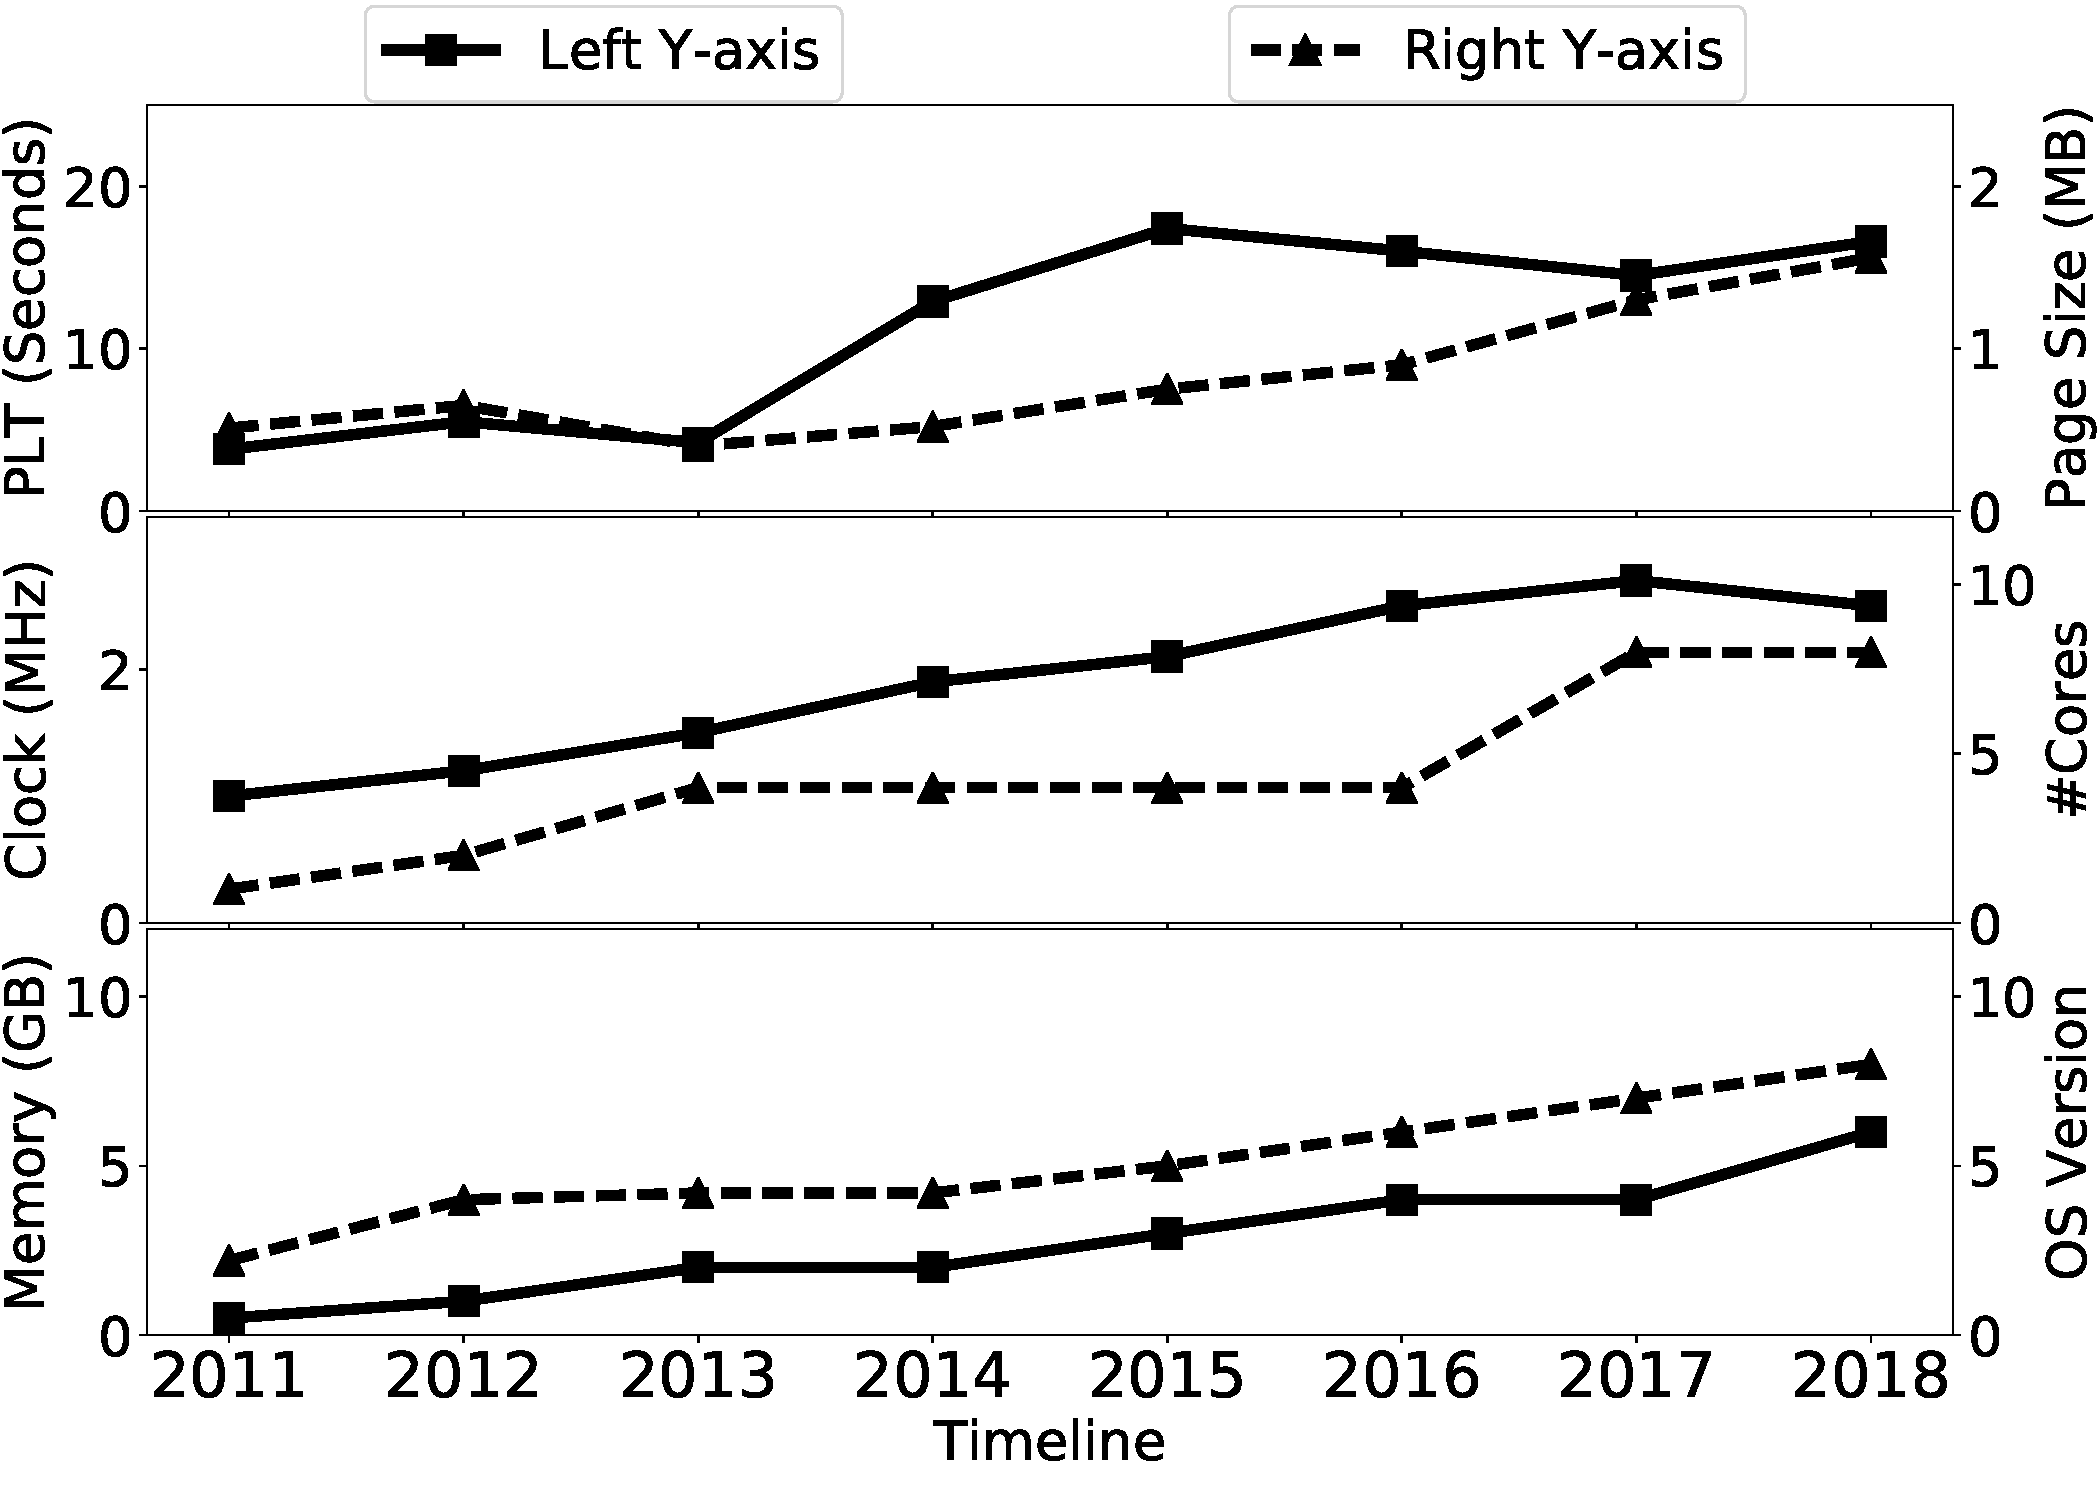
\includegraphics[width=0.85\linewidth]{sections/evolv}
\vspace{-0.3cm}
\caption{Evolution of webpage performance and device parameters over last 8 years. The growth in device performance is not on par with the growth of application demands.}
\label{fig:evolv}
\vspace{-0.6cm}
\end{figure}

Traditional network resource provisioning is based on QoS parameters (such as network throughput, latency, and loss) rather than QoE. 
Also, the smartphone manufacturers does not consider the QoE of applications while enhancing the device parameters.
Because of this, smartphones are not able to cope with the QoE requirements of applications (Fig. \ref{fig:evolv}).
Based on the pageload history \cite{htarch} and device data mined from over 480 Android smartphone specifications over the past 8 years, we find that page load times increased by 4$\times$ despite the improvement in device hardware (clock: 1Ghz to 2.7Ghz, memory: 512MB to 6GB, cores: 2 to 8) and network (3G to 4G and 802.11n to 802.11ac).
Therefore, QoE based design trends of network resource provisioning and device hardware enhancement could potentially improve the experience of these applications.

In this work, we aim to improve the QoE of Internet-based mobile applications.
To achieve this, we evaluate the QoE of three popular applications --- Web browsing, Video Streaming, and Video Telephony. 
In particular, we study the network- and device-side bottlenecks and make an effort to improve the QoE of these applications.

In the first part of our work, we focus on QoE based network resource provisioning to address network-side bottlenecks.
Recent success of using machine learning (ML) in networking enabled several network optimizations for QoE management.
For example, network administrators map traditional QoS parameters to QoE using ML algorithms and control network resources according to the end-user QoE. 
To achieve this, the prior work collects the QoE information from applications and corresponding network statistics to train the ML model. 
However, majority of the existing work rely on applications to get the ground-truth, use inappropriate QoE metrics, not scalable across diverse applications (\S\ref{MOTIVATION}).
To solve this problem, we systematically study the limitations of prior work. We then propose a generic QoE prediction model by using scalable and content independent objective QoE metrics.

In the second part of our work, we study the impact of different device configurations on QoE to find the root cause of device-side bottlenecks.
Given that widely different phones with very different price points are available in the market, a natural question arises: how much of an application's QoE depends on the phone's hardware specs.
This question is specifically important given that it is well known that compute is a key performance bottleneck for mobile applications such as browsing \cite{nejati2016depth}. However, it is not clear which aspect of compute/hardware specification is significant to performance. Knowing which hardware component has the most impact on end-user performance is crucial to designing better phones under a budget.

To address the question posed, we characterize the QoE of common mobile applications under four different hardware components: (1) clock frequency, (2) memory, (3) number of cores, and (4) Android governors. (The governors control the CPU frequency to achieve a good trade off between application performance and power consumption.) Our goal is to understand how each of these device parameters affect QoE of three of the most popular mobile applications: Web browsing, video streaming, and video telephony.

In summary, our contributions and findings are following:

\begin{itemize}
\item We identify the limitations of prior work on video QoE modeling. We propose scalable and content independent QoE metrics and study three popular video telephony applications -- Skype, Hangouts, and FaceTime with diverse network conditions (\S \ref{label:design}). \\
\item We propose a scalable and application independent video QoE prediction model and achieve a median 90\% accuracy (\S \ref{label:model}).
\item We microbenchmark the QoE of three popular mobile Internet applications--- Web browsing, video streaming, and video telephony with different device parameters. We find that Web browsing is most sensitive to device hardware whereas video applications are exploiting specialized hardware accelerators (\S\ref{intro}). 
\item Taking inspiration from video applications, we offload certain browsing computation onto DSP coprocessor opportunistically and achieve 18.5\% improvement in speeding up page loads with 4$\times$ reduction in energy consumption (\S \ref{sec:energy}).
\end{itemize}

